\documentclass[letterpaper,10pt]{article}
\usepackage[top=2cm, bottom=1.5cm, left=1cm, right=1cm]{geometry}
\usepackage{amsmath, amssymb, amsthm, graphicx, enumitem, tikz}
\usetikzlibrary{calc, patterns}
\usepackage{fancyhdr}
\pagestyle{fancy}

\lhead{\today}
\chead{Algebraic Structures HW6}
\rhead{Justin Hood}

\newcommand{\Z}{\mathbb{Z}}
\newcommand{\Q}{\mathbb{Q}}
\newcommand{\R}{\mathbb{R}}
\newcommand{\C}{\mathbb{C}}
\newtheorem{lem}{Lemma}

\begin{document}
\begin{description}
\item[Question 3.] Let $L: \R^2 \to \R^2$ with
\[L\begin{pmatrix}
x\\y
\end{pmatrix}=\begin{pmatrix}
x\cos(\theta)+y\sin(\theta) \\ -x\sin(\theta)+y\cos(\theta)
\end{pmatrix} \]
\begin{enumerate}[label=\alph*.]
\item We write the matrix of $L$ using the basis $\begin{pmatrix}
1\\0
\end{pmatrix},\begin{pmatrix}
0\\1
\end{pmatrix} $ as,
\[L=\begin{bmatrix}
\cos(\theta) & \sin(\theta)\\
-\sin(\theta) & \cos(\theta)
\end{bmatrix} \]
We note that this is the rotation matrix in two dimensions.
\item When $\theta\neq 0$, we consider how the matrix affects a given vector in the plane. We see that the matrix will actually rotate a vector in the plane by $-\theta$. This is shown below, when the operation,
\[L\begin{pmatrix}
1\\0
\end{pmatrix}=\begin{bmatrix}
\cos(\theta) & \sin(\theta)\\
-\sin(\theta) & \cos(\theta)
\end{bmatrix}\begin{pmatrix}
1\\0
\end{pmatrix}=\begin{pmatrix}
\cos(\theta)\\-\sin(\theta)
\end{pmatrix}\]
Is applied with $\theta=\frac{\pi}{4}$.
\begin{center} 
	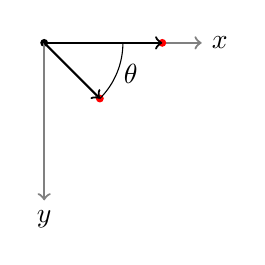
\begin{tikzpicture}
    \coordinate (origo) at (0,0);
	\coordinate (why) at (-1,0);
	\coordinate (ex) at (1,0);
	\coordinate (pivot) at (.7071067,-.7071067);
    % draw axes
    \fill[black] (origo) circle (0.05);
    \draw[thick,gray,->] (origo) -- ++(2,0) node[black,right] {$x$};
    \draw[thick,gray,->] (origo) -- ++(0,-2) node (mary) [black,below] {$y$};
	\fill[red] (1.5,0) circle (0.05);	
	\draw[thick,black,->] (origo) -- ++(1.5,0);
	\fill[red] (0.707106781,-0.707106781) circle (0.05);	
	\draw[thick,black,->] (origo) -- ++(0.707106781,-0.707106781);
	\draw (1,0) arc (0:-45:1cm);
	\draw (1.1,-.4) node{$\theta$};
  	\end{tikzpicture}
\end{center}
As we can see, the vector is rotated 45 degrees in the negative direction.
\item Given the nature of the matrix, we expect that the matrix will have invariant directions when $\theta=0$ and $\theta=\pi$. This corresponds to a rotation of $0$ and $180$ degrees, or coefficients $-1,1$ acting on the vector itself.
\item Next, we attempt to find the eigenvalues of $L$ by solving for the characteristic equation. So,
\begin{align*}
\begin{vmatrix}
\cos(\theta)-\lambda & \sin(\theta)\\ -\sin(\theta) & \cos(\theta)-\lambda
\end{vmatrix} &= (\cos(\theta)-\lambda)(\cos(\theta)-\lambda)-(-\sin^2(\theta))\\
&=\cos^2(\theta)-2\cos(\theta)\lambda+\lambda^2+\sin^2(\theta)\\
0&=\lambda^2-2\cos(\theta)\lambda+1
\end{align*}
Solving for lambda, 
\[\lambda=\frac{2\cos(\theta)\pm\sqrt{4\cos^2(\theta)-4}}{2}=\cos(\theta)\pm\sqrt{-\sin^2(\theta)}\]
Which has no real solutions. However, by allowing $i=\sqrt{-1}$, we may find the solutions to be,
\[\lambda_{1,2}=\cos(\theta)\pm i\sin(\theta)\]
\end{enumerate}
\item[Question 4.] Let $L:\R^3\to \R^3$ where,
\[L\begin{pmatrix}
x\\y\\z
\end{pmatrix}=\begin{pmatrix}
x+y\\x+z\\y+z
\end{pmatrix} \]
\begin{enumerate}[label=\alph*.]
\item Now, let $e_i$ be a vector of all zeros, save a one in the $i^{th}$ position. We now compute,
\begin{align*}
L\begin{pmatrix}
1\\0\\0
\end{pmatrix} &= \begin{pmatrix}
1\\1\\0
\end{pmatrix}\\
L\begin{pmatrix}
0\\1\\0
\end{pmatrix} &= \begin{pmatrix}
1\\0\\1
\end{pmatrix} \\
L\begin{pmatrix}
0\\0\\1
\end{pmatrix} &= \begin{pmatrix}
0\\1\\1
\end{pmatrix}
\end{align*}
\item We now consider the matrix, $M=\begin{pmatrix}
m_1^1 & m_2^1 & m_3^1\\
m_1^2 & m_2^2 & m_3^2\\
m_1^3 & m_2^3 & m_3^3
\end{pmatrix}$ From this, we note that $Me_i$ becomes the vector $\begin{pmatrix}
m_i^1\\m_i^2\\m_i^3
\end{pmatrix} $
\item We now compute the matrix representation of $L$ as,
\[M=\begin{pmatrix}
1 & 1 & 0\\
1 & 0 & 1\\
0 & 1 & 1
\end{pmatrix}\]
\item We now compute the eigenvalues and vectors of $M$. So,
\begin{align*}
\begin{vmatrix}
1-\lambda & 1 & 0\\
1 & -\lambda & 1\\
0 & 1 & 1-\lambda
\end{vmatrix} &= (1-\lambda)(-\lambda(1-\lambda)-1)-(1-\lambda)\\
&= -\lambda(1-\lambda)^2-(1-\lambda)-(1-\lambda)\\
&= -\lambda+2\lambda^2-\lambda^3-2+2\lambda\\
&=-\lambda^3+2\lambda^2+\lambda-2\\
0 &= -(\lambda-2)(\lambda-1)(\lambda+1)
\end{align*}
So, $\lambda=2,1,-1$. Then,
\begin{align*}
\begin{pmatrix}
1-2 & 1 & 0\\
1 & -2 & 1\\
0 & 1 & 1-2
\end{pmatrix} &= \begin{pmatrix}
-1 & 1 & 0\\
1 & -2 & 1\\
0 & 1 & -1
\end{pmatrix}\\
&= \begin{pmatrix}
-1 & 0 & 1\\
0 & 1 & -1\\
0 & 0 & 0
\end{pmatrix}
\end{align*}
So, we see that $x=z$ and $y=z$. Thus,
\[\lambda=2\Rightarrow v_2=\begin{pmatrix}
1\\1\\1
\end{pmatrix}\]
Next,
\begin{align*}
\begin{pmatrix}
1-1 & 1 & 0\\
1 & -1 & 1\\
0 & 1 & 1-1
\end{pmatrix} &= \begin{pmatrix}
0 & 1 & 0\\
1 & -1 & 1\\
0 & 1 & 0
\end{pmatrix}\\
&= \begin{pmatrix}
0 & 1 & 0\\
1 & 0 & 1\\
0 & 0 & 0
\end{pmatrix}
\end{align*}
So, we see that $x=-z$ and $y=0$. Thus,
\[\lambda=1\Rightarrow v_1=\begin{pmatrix}
1\\0\\-1
\end{pmatrix}\]
Finally,
\begin{align*}
\begin{pmatrix}
1+1 & 1 & 0\\
1 & 1 & 1\\
0 & 1 & 1+1
\end{pmatrix} &= \begin{pmatrix}
2 & 1 & 0\\
1 & 1 & 1\\
0 & 1 & 2
\end{pmatrix}\\
&= \begin{pmatrix}
1 & 0 & -1\\
0 & 1 & 2\\
0 & 0 & 0
\end{pmatrix}
\end{align*}
So, we see that $x=z$ and $y=-2z$. Thus,
\[\lambda=2\Rightarrow v_2=\begin{pmatrix}
1\\-2\\1
\end{pmatrix}\]
\end{enumerate}
\item[Question 8.] Let,
\[M=\begin{pmatrix}
a & b\\
c & d
\end{pmatrix}\]
Then,
\begin{align*}
\begin{vmatrix}
a-\lambda & b\\
c & d-\lambda
\end{vmatrix} &= (a-\lambda)(d-\lambda)-bc\\
&=ad-a\lambda-d\lambda+\lambda^2-bc\\
P_M(\lambda)&=\lambda^2-a\lambda-d\lambda+ad-bc
\end{align*}
Now, let us set $\lambda=M$ and compute,
\[P_M(M)=\begin{pmatrix}
a^2+bc & ab+bd\\
ac+cd & bc+d^2
\end{pmatrix}-\begin{pmatrix}
a^2 & ab\\
ac & ad
\end{pmatrix}-\begin{pmatrix}
ad & bd\\
cd & d^2
\end{pmatrix}+\begin{pmatrix}
ad-bc & 0\\
0 & ad-bc
\end{pmatrix}=\begin{pmatrix}
0 & 0\\
0 & 0
\end{pmatrix} \]
So, we see that $P_M(M)=0$ for $2\times 2$ matrices. We now consider the space of $3\times 3$ matrices. For simplicity, we consider matrices of the form,
\[\begin{pmatrix}
a & 0 & 0\\
0 & b & 0\\
0 & 0 & c
\end{pmatrix}\] Which for convenience we will write as vectors of the form,
\[\begin{pmatrix}
a\\b\\c
\end{pmatrix}\]
As before, we compute the equation,
\[P_M(\lambda)=abc-ac\lambda-bc\lambda+c\lambda^2-ab\lambda+a\lambda^2+b\lambda^2-\lambda^3\]
So, we may compute,
\[P_M(M)=\begin{pmatrix}
abc\\abc\\abc
\end{pmatrix}-\begin{pmatrix}
a^2c\\abc\\ac^2
\end{pmatrix}-\begin{pmatrix}
abc\\b^2c\\bc^2
\end{pmatrix}+\begin{pmatrix}
a^2c\\b^2c\\c^3
\end{pmatrix}-\begin{pmatrix}
a^2b\\ab^2\\abc
\end{pmatrix}+\begin{pmatrix}
a^3\\ab^2\\ac^2
\end{pmatrix}+\begin{pmatrix}
a^2b\\b^3\\bc^2
\end{pmatrix}-\begin{pmatrix}
a^3\\b^3\\c^3
\end{pmatrix} \]
\[=\begin{pmatrix}
0 & 0 & 0\\
0 & 0 & 0\\
0 & 0 & 0
\end{pmatrix}\]
So, we see that the equivalence $P_M(M)=0$ seems to hold for $3\times 3$ matrices.
\end{description}
\end{document}
